\section{Introduction}
\label{sec:intro}

The year 2030 will mark the start of the High-Luminosity phase of the Large
Hadron Collider (HL-LHC)~\cite{HLLHC}, which will deliver proton--proton
collisions at an unprecedented luminosity. The resulting data
volume and the severe pileup---of order $200$ simultaneous interactions per
bunch crossing---demand a new generation of reconstruction algorithms. To cope
with these conditions the CMS experiment will replace its endcap calorimeters
with the High-Granularity Calorimeter (HGCAL)~\cite{HGCALTDR}, a sampling
calorimeter with roughly six million channels arranged in about fifty
longitudinal layers. Its fine transverse and longitudinal segmentation capture detailed three-dimensional structure of electromagnetic and hadronic
showers. It also makes traditional calorimeter clustering impractical and
motivates dedicated clustering algorithms.

\begin{figure*}[!tp]
  \centering
  \begin{subfigure}[b]{0.38\textwidth}
    \centering
    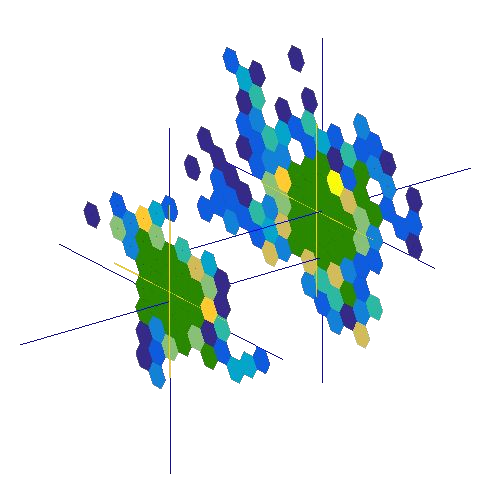
\includegraphics[height=4.6cm,keepaspectratio]{figures/VISUAL_rechits.png}
    \caption{RecHits and LayerClusters}
    \label{fig:rechits-a}
  \end{subfigure}
  \hspace{0.04\textwidth}
  \begin{subfigure}[b]{0.56\textwidth}
    \centering
    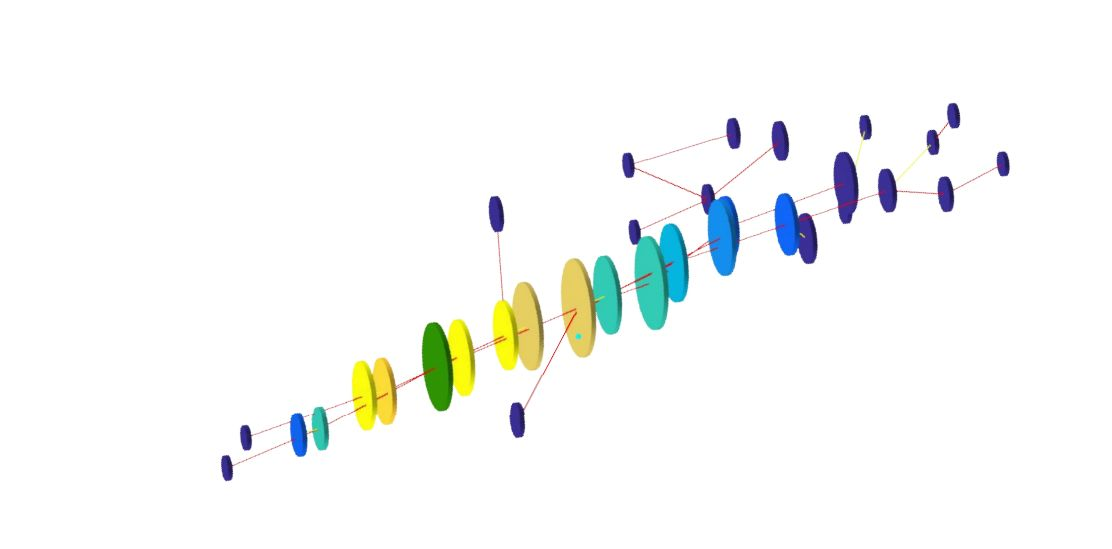
\includegraphics[height=4.6cm,keepaspectratio]{figures/VISUAL_tracks.jpg}
    \caption{LayerClusters linked into a Trackster}
    \label{fig:rechits-b}
  \end{subfigure}
  \caption{The HGCAL reconstruction chain. (a) Calibrated energy deposits
  (RecHits) of two photon showers. CLUE groups them by layer into
  two-dimensional LayerClusters.
  (b) \cluethreed{} links LayerClusters across layers into a
  three-dimensional Trackster; the red lines are the nearest-higher links that
  build the shower.}
  \label{fig:rechits}
\end{figure*}

The Clustering of Energy (CLUE) algorithm~\cite{Rovere2020clue} was developed for this purpose: it is a fast, parallel, energy density-based clustering algorithm. It groups HGCAL energy deposits into physics objects such as photons and
electrons. In the CMS reconstruction, CLUE and its three-dimensional extension
\cluethreed{} sit inside The Iterative Clustering (TICL)
framework~\cite{TICL}, which builds objects in stages
(Fig.~\ref{fig:rechits}): individual calorimeter hits (\emph{RecHits}) are first
grouped per layer by CLUE into two-dimensional \emph{LayerClusters} (LCs);
\cluethreed{} then links LayerClusters from multiple layers into three-dimensional
\emph{Tracksters}; and a subsequent linking step associates Tracksters into the
final TICL candidates. The Monte Carlo truth is described by an analogous chain,
in which a generated particle (\emph{CaloParticle}) is mapped to a
\emph{SimTrackster} that collects the LayerClusters that belong to it.
Reconstruction performance is measured by comparing reconstructed Tracksters to
SimTracksters through their shared energy.

An important \cluethreed{} assumption: the neighbour search that links layer
clusters across layers is performed in a coordinate system projected from
the interaction point (IP), therefore shower travelling outward
from the CMS centre keeps fixed projected position layer to layer. This
holds for \emph{prompt} particles produced at the beamline, but it doesn't need to for
the class of \emph{long-lived particles} (LLPs) predicted by many extensions of
the Standard Model~\cite{LLPreview}. Rather than decaying within a few
millimetres of IP, an LLP can travel longer distance in the detector before decaying, producing \emph{displaced}, non-pointing
particles. A representative signature is a dark shower in which
long-lived dark hadrons decay to Standard Model photons far from the beamline. Because these showers do not point back to
the origin, they may violate exactly the assumption on which \cluethreed{}
relies.

The goal of this project is to determine
is \cluethreed{} capable of clustering the energy deposits from such
novel topologies, to measure the expected performance degradation as a function
of the distance from IP to where LLP decays, and to explore an alternative algorithm. We restrict the study to
neutral \emph{photons}: photons whose trajectory is not curved by the CMS magnetic field, so
they go in straight lines and their displacement is unambiguously defined; they also do not interact in the tracker before
reaching the calorimeter. This isolates the calorimeter clustering behaviour
from tracking and magnetic-field effects and provides the cleanest possible test
of the origin assumption.

The remainder of this report is organized as follows. We first define the
displacement observables and describe how they are defined for reconstructed objects, then present the displaced-photon Monte Carlo
production and the performance metrics. After reviewing how \cluethreed{} works,
with emphasis on the origin assumption, we present the single-photon efficiency,
the two-shower merging behaviour, and the performance under pileup, before
comparing \cluethreed{} against the alternative algorithm \cluestering{} and
concluding.
